\scanpage{15}
\[
\underset{\substack{\unsure{\wr\Vert|\Vert|\simeq}\\\mathbb Z/4\mathbb Z}}{\Gamma=(\mathbb Z/5\mathbb Z)^*}
\]
\diagram{\begin{tikzcd}[ampersand replacement=\&,column sep=small,row sep=small]
\mu_5 \arrow[d,dash] \& {\supset}\ \mu_5^* \arrow[d,dash]\& \deleted{\unsure{B}}\ \tau=\mu_5^*/\beta\\
\underset{\unsure{(\mathrm{id},d)|(0,d)|(\alpha,\alpha')}}{\operatorname{Spec}\mathbb Z} \arrow[r,phantom,"\unsure{\supset|\longrightarrow|\longleftarrow}" description] \& \mathbb Z[\tfrac15] \arrow[ur,dash] \&
\end{tikzcd}}
fini étale de \deleted{\unsure{degré}} rang 4 sur $\mathbb Z[\frac15]$ ; \deleted{\unsure{galoisien}} Galoisien de groupe $\Gamma$

engendré par $\unsure{\zeta|\xi}+\bar\zeta=\zeta+\zeta^{-1}=\unsure{\eta|\gamma}$
\inserted{$\zeta$\ $\rightarrow$ racine primitive universelle}

\margin{deux générateurs 2 et 3 \inserted{$=-2$} mod 5. un élément \inserted{$-1$} d'ordre 2 $-1$ ou 4 mod 5. un élément d'ordre 1 \quad 1 mod 5}
Sur $\mu_5(S)$ l'effet est $\zeta\mapsto\zeta^2$ ou $\zeta\mapsto\zeta^{-2}=\zeta^3$ resp.
\[
\begin{aligned}\zeta&\mapsto\zeta^{-1}=\zeta^4\\
\zeta&\mapsto\zeta\end{aligned}
\]
\diagram{\begin{tikzcd}[ampersand replacement=\&,row sep=small,column sep=1pt]
B\arrow[d,dash]\&{\supset B^\Gamma}\\ A\&
\end{tikzcd}}
\[
\left\{\begin{aligned}B&=A[\zeta]/\deleted{\unsure{T=}}\\
&A[T]/(1+T+T^2+T^3+T^4)
\end{aligned}\right.
\]
\[
T\mapsto T^4
\]
\figure{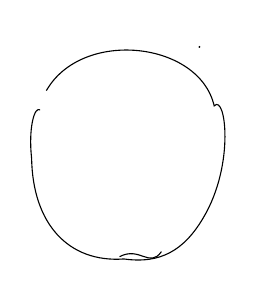
\begin{tikzpicture}[scale=.72]
\draw (.22,2.25) .. controls (.85,3.35) and (2.92,3.12) .. (3.18,1.98)
.. controls (3.38,2.20) and (3.55,.95) .. (2.99,.01)
.. controls (2.65,-.57) and (2.23,-.81) .. (1.59,-.72)
.. controls (.60,-.79) and (-.02,-.09) .. (-.04,1.05)
.. controls (-.10,1.59) and (.01,1.98) .. (.11,1.91);
\draw (1.51,-.68) .. controls (1.87,-.49) and (2.04,-.89) .. (2.25,-.59);
\fill (2.92,3.02) circle (.018);
\end{tikzpicture}}

\({}_nU\) étale de rang $n$ sur $\mathbb Z$ si on prend \deleted{\unsure{\({}_nU\)}} $\mu_n$ \uline{tordu} par $T$
\diagram{\begin{tikzcd}[ampersand replacement=\&,row sep=small,column sep=small]
\&\mu_n\arrow[d,phantom,"\cup"]\&\\
\varphi(n)\arrow[dr,dash]\arrow[r,dash]\&\mu_n^*\arrow[d]\&(\mathbb Z/n\mathbb Z)^*\\
\&S\&
\end{tikzcd}}
\[
\zeta\unsure{\mapsto|\vdash}\zeta^{-1}
\]
\[
\begin{aligned}
\beta(T)&=T^{-1}=T^4=-(1+T+T^2+T^3)\\
\beta(T^2)&=T^{-2}=T^3\\
\beta(T^3)&=T^{-3}=T^2\\
\beta(T^4)&-
\end{aligned}
\]
\[
1=T^0/T\quad T\quad T^2\quad T^3
\]
\diagram{\begin{tikzcd}[ampersand replacement=\&,row sep=small,column sep=small]
\text{gp}\&\mu_n^T\arrow[d,phantom,"\cup"]\&{\subset U}\\
\text{pas groupe}\&\mu_n^{*T}\arrow[d,"\substack{\text{étale}\\\text{rang }2}"']\&{\subset U}\arrow[d,"\operatorname{Tr}_{K/O}"]\&\zeta+\zeta\\
\&\mathbb V_n^T=V_n\arrow[d,"\substack{\text{étale}\\\text{rang }\varphi(n)/2}"']\&{\subset O}\\
\&S\&
\end{tikzcd}}
\[
\underset{\displaystyle\prod(p_i^{\alpha_i}-p_i^{\alpha_i-1})}{\underset{\Vert}{\varphi(n)}}\qquad
\begin{aligned}
\beta(c_0+c_1T+c_2T^2+c_3T^3)&\deleted{\unsure{=c_0+}}\\
&=c_0\unsure{+|-}c_1(-1+T+T^2+T^3)\\
&\qquad{}+c_2T^3+c_3T^2\\
&=(c_0-c_1)-c_1T+(c_3-c_1)T^2+(c_2-c_1)T^3\\
&\overset{?}{=}c_0+c_1T+c_2T^2+c_3T^3
\end{aligned}
\]
\[
(\mathbb Z/n\mathbb Z)^*\ni-1\qquad\mu_n\subset G_m
\]
\[
p^{n}-p^{n-1}=p^{n-1}(p-1)
\]
\diagram{\begin{tikzcd}[ampersand replacement=\&,row sep=small,column sep=small]
\mu_n^*\arrow[d] \& {\subset G_m}\arrow[d,"\unsure{\rho|c}"]\\
\mathbb V_n \& {\subset\mathbb E^1}
\end{tikzcd}}
\[
\rho(\lambda)=\lambda+\lambda^{-1}\qquad c_1=0\qquad c_2=c_3
\]
\[
\zeta+\zeta^{\deleted{\unsure{2}}-1}\ \bigg|\ \begin{aligned}\frac{p-1}{2}&=2\\ &\cos\end{aligned}
\qquad c_0+c_2(T^2+T^3)
\]
\[
\begin{aligned}
1+\zeta+\zeta^2+\zeta^3+\zeta^4&=0\\
\zeta+\zeta^{-1}&=\deleted{\unsure{\alpha}}\gamma
\end{aligned}
\qquad
\begin{aligned}
\operatorname{Tr}\gamma&=\gamma+\gamma^\sigma=\zeta+\zeta^{-1}+\zeta^2+\zeta^{-2}\\
&=\zeta+\zeta^2+\zeta^3+\zeta^4=-1\\
N\gamma&=\gamma\gamma^{\unsure{\sigma|\alpha}}=(\zeta+\zeta^{-1})(\zeta^2+\zeta^{-2})=
\end{aligned}
\]
% archive sheet number: 14
